%% ----------------------------------------------------------------
%% Article.tex
%% ---------------------------------------------------------------- 
\documentclass{ecsarticle}     % Use the Article Style
\graphicspath{{Figures/}}   % Location of your graphics files
\usepackage{natbib}            % Use Natbib style for the refs.
\hypersetup{colorlinks=false}   % Set to false for black/white printing
\input{Definitions}            % Include your abbreviations

\usepackage[nodayofweek]{datetime}
\usepackage{listings}
\usepackage{color}
\usepackage{fontenc}
\usepackage{multirow}
\usepackage{amsmath}


\usepackage{graphicx}



%% ----------------------------------------------------------------
\begin{document}
%TC:ignore
\frontmatter
\title      {COMP6036: Advanced Machine Learning\\
            Feature Selection Challenge}
      
\addresses  {\deptname\\\univname}
\authors                 {\href{mailto:ajr2g10@ecs.soton.ac.uk}{Ashley J. Robinson}\\\href{mailto:ajr2g10@ecs.soton.ac.uk}{ajr2g10@ecs.soton.ac.uk}}

\date       {\today}
\subject    {}
\keywords   {}
\maketitle
%% ----------------------------------------------------------------


\begin{abstract}
All algorithms implemented in this report is written by the author for the MATLA programming language.
Initial testing with a linear perceptron using all features in the input space yields good results on the dexter and gisette datasets.
The objective is to further optimise the performance on these datasets. 
\end{abstract}

%TC:endignore
\mainmatter


\section{Introduction}

Each dataset has been divided in three section for training, validation and test submission.
The final partition labels remain hidden from the development process.
The discrete class labels, $t$, and the classifier outputs, $y$, are described by equation~\eqref{eqn:output}.
Keeping to these output values requires using the thresholding function $\Theta$ in equation~\eqref{eqn:theta}. 
Everything implemented has been developed from scratch for the MATLAB programming language. 


\begin{equation}
	y,t \in \{-1,+1\}
	\label{eqn:output}
\end{equation}

\begin{equation}
	\Theta(a) = \left\{ 
      \begin{array}{l}
         +1,\:a > 0\\
         -1,\:a \leq 0\\
      \end{array} \right.	
	\label{eqn:theta}
\end{equation}

\section{Classifier Build and Test}

Artificial Neural Networks (ANNs) have been chosen as the classifier architectures.
ANNs are efficient learning machines with biological inspiration~\citep{bishop06pattern}. 
They are parametric models which can be adapted during supervised training and are scalable in complexity.
The error space can be considered as a function of parameters and the training data, $E(w|D)$, therefore many different optimisation algorithms can be used can used to train the model. 



\subsection{Perceptron}
\label{sec:perceptron}

Figure~\ref{fig:slp} holds the most simple manifestation of an ANN called a perceptron.
Each feature of an input pattern is weighted and then summed, along with a bias term, to produce an output.
This output passes through a step activation function for binary classification.
Capable of producing a linear separation boundary the method serves as starting point for further investigation into the data.
The architecture is vectorised in equation.~\eqref{eqn:slp_mat} to classify an entire dataset. 
The offset parameter, $b$, is included in the matrix and the input patterns are fixed with the unit feature to assist with training the classifier. 

Batch training is done iteratively using equation~\eqref{eqn:slp_learn} where the error between the output and labels is propagates back to the weights using the transpose of the input patterns.
A training parameter, $\eta$, hes been manually tuned to $10^{-4}$.
Figure~\ref{fig:slp_train} shows the performance on the dexter dataset over the training process.
Tested upon the available datasets the only two reasonable performances were on dexter and gisette which is shown in tables~\ref{tab:slp_dexter} and~\ref{tab:slp_gisette} respectively.
All code for the perceptron is held in appendix~\ref{sec:slp_appendix}

\begin{figure}[ht]
   \centering
    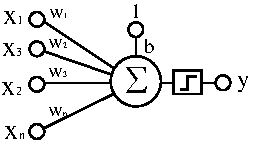
\includegraphics[width = 6cm]{SLP.pdf}
   \caption{Perceptron architecture.}
   \label{fig:slp}
\end{figure}

\begin{equation}
   \textbf{Y} = \Theta ( \textbf{X}.\textbf{W})
   \label{eqn:slp_mat}
\end{equation}

\begin{equation}	
	\textbf{W}_{t+1} = \textbf{W}_t + \mathbf{\eta}*(\mathbf{Y}-\mathbf{T})\mathbf{X}^T
	\label{eqn:slp_learn}
\end{equation}


\begin{figure}[ht]
   \centering
    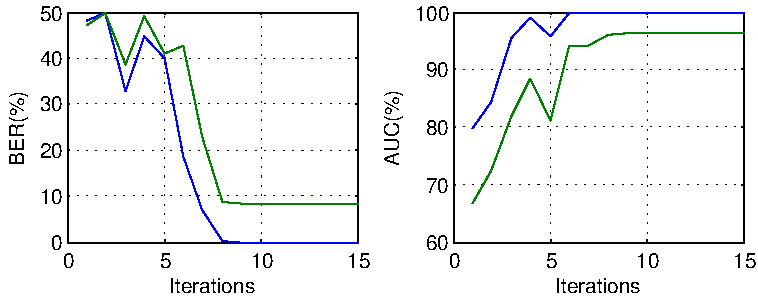
\includegraphics[width = 14cm]{SLP_train.pdf}
   \caption{Perceptron training on the dexter dataset.}
   \label{fig:slp_train}
\end{figure}


\begin{table}[h]
	\centering
	\begin{tabular}{|l|l|l|l|} \hline
     			& Train & Valid & Test \\ \hline
		BER & 0.0000 & 0.0633 & 0.0735 \\ \hline
		AUC & 1.0000 & 0.9779 & 0.9767 \\ \hline
	\end{tabular}
	\caption{Perceptron results on dexter. Submission ID 5518 in Appendix~\ref{sec:id}.}
	\label{tab:slp_dexter}
\end{table}

\begin{table}[h]
	\centering
	\begin{tabular}{|l|l|l|l|} \hline
     			& Train & Valid & Test \\ \hline
		BER & 0.0445 & 0.0430 & 0.0432 \\ \hline
		AUC & 0.9889 & 0.9894 & 0.9907 \\ \hline
	\end{tabular}
	\caption{Perceptron results on gisette. Submission ID 5518 in Appendix~\ref{sec:id}.}
	\label{tab:slp_gisette}
\end{table}






\subsection{Multi Layer Perceptron (MLP)}
Section~\ref{sec:perceptron} can be expanded by concatenating the architecture to produce a multi layer perceptron.
They contain hidden layers and when used with non-linear activation functions can produced a non-linear separation boundary~\citep{bennett01ml}.
Only one hidden layer is implemented for simplicity as shown in figure~\ref{fig:mlp}.
The hidden nodes use an offset $tanh$ and output uses the $\Theta$ function.


When testing the MLP all the features are used with $50$ hidden nodes.
Table~\ref{tab:mlp_dexter} is trained using a value of $\eta$ set to $10^{-4}$ yet shows no improvement.
The training set is learnt quickly and no improvement is shown in the validation set.
Table~\ref{tab:mlp_gisette} does show an improvement over the perceptron with $\eta$ set to $10^{-5}$.
The taring set is not full learnt and a steady increase in performance is shown during training in figure~\ref{fig:mlp_train}.
Code for this implementation is held in appendix~\ref{sec:mlp_appendix}


\begin{figure}[ht]
   \centering
    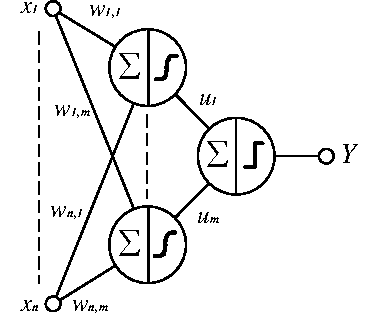
\includegraphics[width = 7cm]{MLP.pdf}
   \caption{MLP architecture.}
   \label{fig:mlp}
\end{figure}

\begin{equation}
   y = \Theta \left(b + \sum_{i=1}^{m} u_i \tanh \left(c_i + \sum_{j=1}^{n} x_j w_{j,i}\right)  \right) 
   \label{eqn:mlp}
\end{equation}

\begin{figure}[ht]
   \centering
    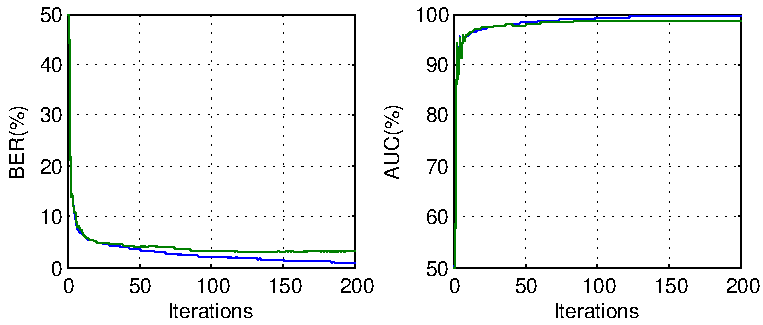
\includegraphics[width = 14cm]{MLP_Train.pdf}
   \caption{MLP training on the gisette dataset.}
   \label{fig:mlp_train}
\end{figure}


\begin{table}[h]
	\centering
	\begin{tabular}{|l|l|l|l|} \hline
     			& Train & Valid & Test \\ \hline
		BER & 0.0120 & 0.0280 & 0.0312 \\ \hline
		AUC & 0.9955 & 0.9864 & 0.9839 \\ \hline
	\end{tabular}
	\caption{MLP results on gisette. Submission ID 5549 in Appendix~\ref{sec:id}.}
	\label{tab:mlp_gisette}
\end{table}




\section{Feature Selection}




\section{Results}

\section{Conclusions}


\newpage

%TC:ignore
\bibliographystyle{ecs}
\bibliography{references}



\backmatter
\begin{appendix}

\newpage


\section{Submission ID URLs}
\label{sec:id}
\begin{itemize}
	\item 5518: \href{http://www.nipsfsc.ecs.soton.ac.uk/description/?id=5518}{http://www.nipsfsc.ecs.soton.ac.uk/description/?id=5518}
	\item 5549: \href{http://www.nipsfsc.ecs.soton.ac.uk/description/?id=5549}{http://www.nipsfsc.ecs.soton.ac.uk/description/?id=5549}
\end{itemize}



\definecolor{mygreen}{rgb}{0,0.6,0}
\definecolor{mygray}{rgb}{0.5,0.5,0.5}
\definecolor{mymauve}{rgb}{0.58,0,0.82}

\lstset{ %
  %backgroundcolor=\color{white},   % choose the background color; you must add \usepackage{color} or \usepackage{xcolor}
  basicstyle=\footnotesize,        % the size of the fonts that are used for the code
  breakatwhitespace=false,         % sets if automatic breaks should only happen at whitespace
  breaklines=true,                 % sets automatic line breaking
  captionpos=b,                    % sets the caption-position to bottom
  commentstyle=\color{mygreen},    % comment style
  deletekeywords={...},            % if you want to delete keywords from the given language
  escapeinside={\%*}{*)},          % if you want to add LaTeX within your code
  extendedchars=true,              % lets you use non-ASCII characters; for 8-bits encodings only, does not work with UTF-8
  frame=single,                    % adds a frame around the code
  keepspaces=true,                 % keeps spaces in text, useful for keeping indentation of code (possibly needs columns=flexible)
  keywordstyle=\color{blue},       % keyword style
  language=Matlab,                 % the language of the code
  morekeywords={*,...},            % if you want to add more keywords to the set
  numbers=left,                    % where to put the line-numbers; possible values are (none, left, right)
  numbersep=5pt,                   % how far the line-numbers are from the code
  numberstyle=\tiny\color{black}, % the style that is used for the line-numbers
  rulecolor=\color{black},         % if not set, the frame-color may be changed on line-breaks within not-black text (e.g. comments (green here))
  showspaces=false,                % show spaces everywhere adding particular underscores; it overrides 'showstringspaces'
  showstringspaces=false,          % underline spaces within strings only
  showtabs=false,                  % show tabs within strings adding particular underscores
  stepnumber=1,                    % the step between two line-numbers. If it's 1, each line will be numbered
  stringstyle=\color{mymauve},     % string literal style
  tabsize=4,                       % sets default tabsize to 2 spaces
  title=\lstname                   % show the filename of files included with \lstinputlisting; also try caption instead of title
}



\section{Code Listings}
\subsection{Perceptron}
\label{sec:slp_appendix}
\lstinputlisting[label=lst:slpRun.m,caption=run.m]{../SLP/run.m}
\lstinputlisting[label=lst:slpTrain.m,caption=train.m]{../SLP/train.m}
\lstinputlisting[label=lst:slpTrainGraph.m,caption=trainGraph.m]{../SLP/train_graph.m}
\lstinputlisting[label=lst:slpPredict.m,caption=predict.m]{../SLP/predict.m}
\lstinputlisting[label=lst:slpFeatSelect.m,caption=featSelect.m]{../SLP/feat_select.m}

\subsection{Multi Layer Perceptron}
\label{sec:mlp_appendix}
\lstinputlisting[label=lst:mlpRun.m,caption=run.m]{../MLP/run.m}
\lstinputlisting[label=lst:mlpTrain.m,caption=train.m]{../MLP/train.m}
\lstinputlisting[label=lst:mlpPredict.m,caption=predict.m]{../MLP/predict.m}
\lstinputlisting[label=lst:mlpFeatSelect.m,caption=featSelect.m]{../SLP/feat_select.m}



\end{appendix}

%TC:endignore
\end{document}
%% ----------------------------------------------------------------

